\chapter{Results and Analysis}\label{ch:results}

This chapter presents the performance of GP regression in estimating various
measures based on a simulation study.
The estimation performance of GP regression is compared with that of baseline methods.
The performance is reported for different downsampling factors, where a downsampling
factor of 2 implies that the training data contains half of the samples from the
original signal $F_X$, which has 10 samples per hour.
Additionally, results for both uniform and seasonal sampling are presented.

\section{Target Measures}

In this section, we evaluate the effectiveness of GP regression ("gp") in
estimating specific target measures. These target measures include the one-week mean,
one-day mean, one-hour mean, and time in the target range (TTR).
We compare the estimation performance of GP regression with that of several baseline methods,
including linear regression ("linear"), spline regression ("spline"), overall mean
("overall\_mean"), and naive TTR ("naive\_ttr").

\subsection{One-Week Mean}

Figure \ref{fig:weekly-mean-performance} illustrates the performance of different
methods in estimating the one-week mean under different sampling patterns.
Subfigure \ref{fig:weekly-mean-uniform-sampling-performance} and
\ref{fig:weekly-mean-seasonal-sampling-performance} display the results
for uniform and seasonal sampling, respectively. Within each subfigure, the panels
represent decreasing downsampling factors from left to right.

Performance is presented in terms of confidence or credible interval (CI) width and CI coverage.
CI width represents the width of the estimated 95\% CI for the one-week mean BP value,
measured in mmHg. CI coverage indicates the number of times the true one-week BP
values were covered by the estimated CI over 100 simulations.

Ideally, a method should achieve 95\% CI coverage with a very low CI width,
positioning itself in the upper-left corner of the plot. Achieving 95\% coverage
is considered more critical than having a low width.
Based on this 100 simulation runs, the confidence intervals
of the CI coverage values have been calculated.
Whenever these confidence intervals of the CI coverage
spans across 95\% coverage, the method is deemed adequate.

It is important to note that all plots have the same range of CI coverage values
on the y-axis, but the x-axis range of CI width values varies. As expected,
CI width values increase with larger downsampling factors and with seasonal sampling.
The CI width is capped at 30 mmHg, as larger CIs would have limited practical value.

For the largest downsampling factors, the spline regression method
would produce confidence intervals that exceed this limit and is therefore not
represented in the corresponding panel of subfigure
\ref{fig:weekly-mean-uniform-sampling-performance}.
It appears that the approach used for spline regression produces unstable
estimates during bootstrapping, resulting in very large confidence intervals.


For the one-week mean the overall mean is equivalent to the naive TTR estimate.
Therefore, naive TTR is omitted from this analysis.
All methods perform adequately with uniform sampling.
While linear regression seems to produce the smallest confidence intervals for
the largest downsampling factor, estimates do not improve as notably as for
spline regression and GP regression when more data becomes available.
For downsampling factors below 5, GP regression, linear regression, and spline
regression produce very similar results.

In the presence of seasonal sampling, the overall mean obviously does not
provide good estimates. GP regression generally
comes closest to the target coverage, but for high downsampling factors,
linear regression remains competitive and provides even smaller CI widths.
However, the more data available the more linear regression seems to
diverge from the true BP values. This effects are more pronounced in the face
of extreme seasonal sampling.


In conclusion, both linear and GP regression produce the best one-week mean estimates.
Linear regression is preferable for very high downsampling factors,
while GP regression is recommended for downsampling factors below 5,
corresponding to an average of 2 or more measurements per hour.

\begin{figure}[!htb]
\centering
\begin{subfigure}{\textwidth}
    \centering
    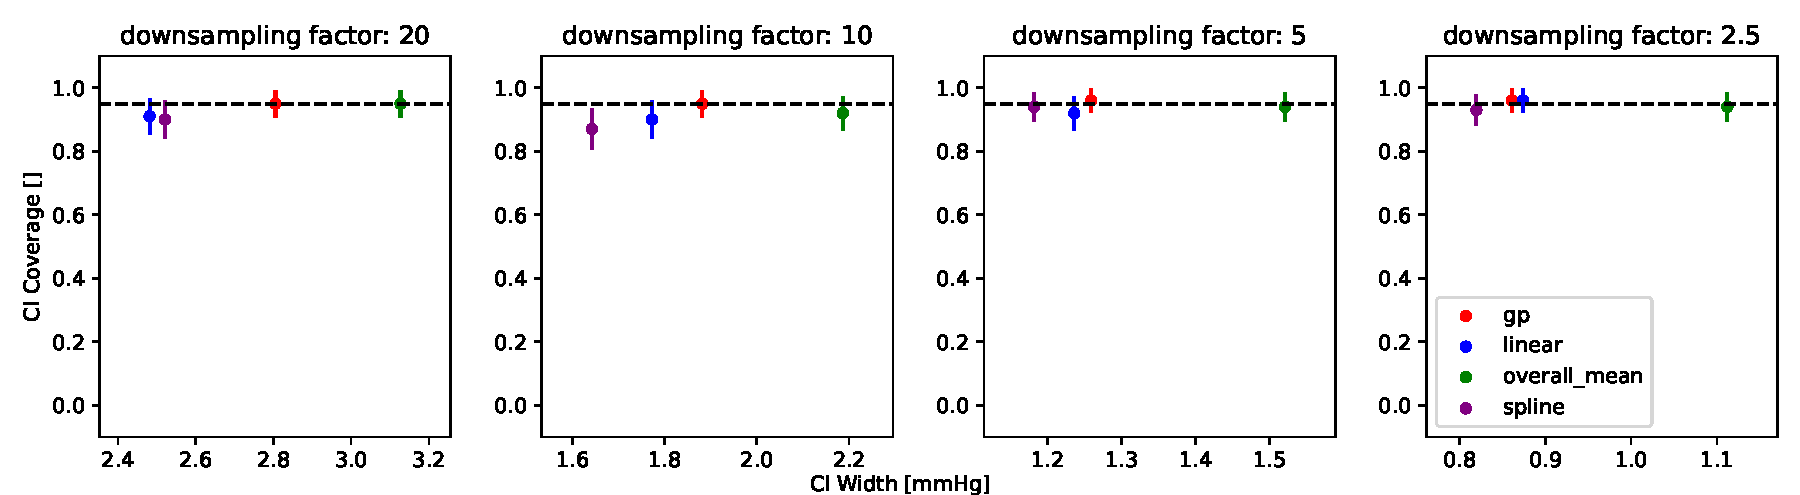
\includegraphics[width=\linewidth]{Pictures/final_experiment_hpdi/overall_mean_eval_sin_rbf_default}
    \caption{One-Week Mean - Uniform Downsampling}
    \label{fig:weekly-mean-uniform-sampling-performance}
\end{subfigure}

\bigskip

\begin{subfigure}{\textwidth}
    \centering
    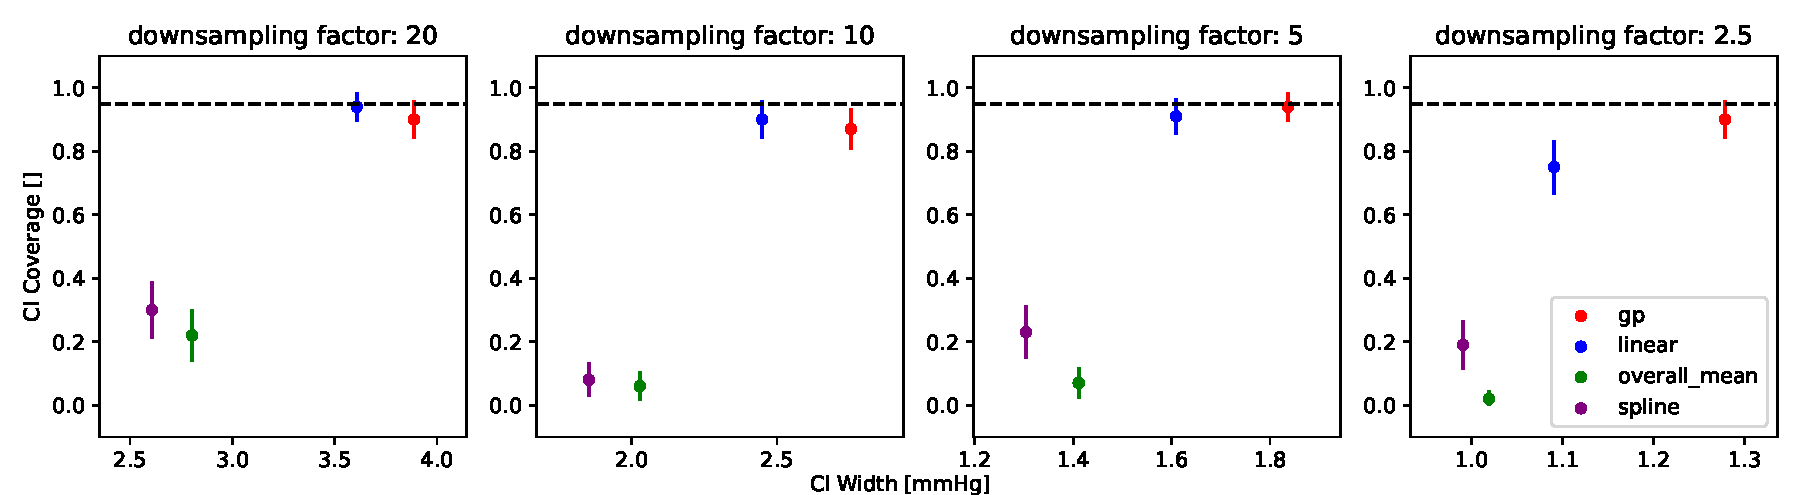
\includegraphics[width=\linewidth]{Pictures/final_experiment_hpdi/overall_mean_eval_sin_rbf_seasonal_default}
    \caption{One-Week Mean - Seasonal Downsampling}
    \label{fig:weekly-mean-seasonal-sampling-performance}
\end{subfigure}

\bigskip

\begin{subfigure}{\textwidth}
    \centering
    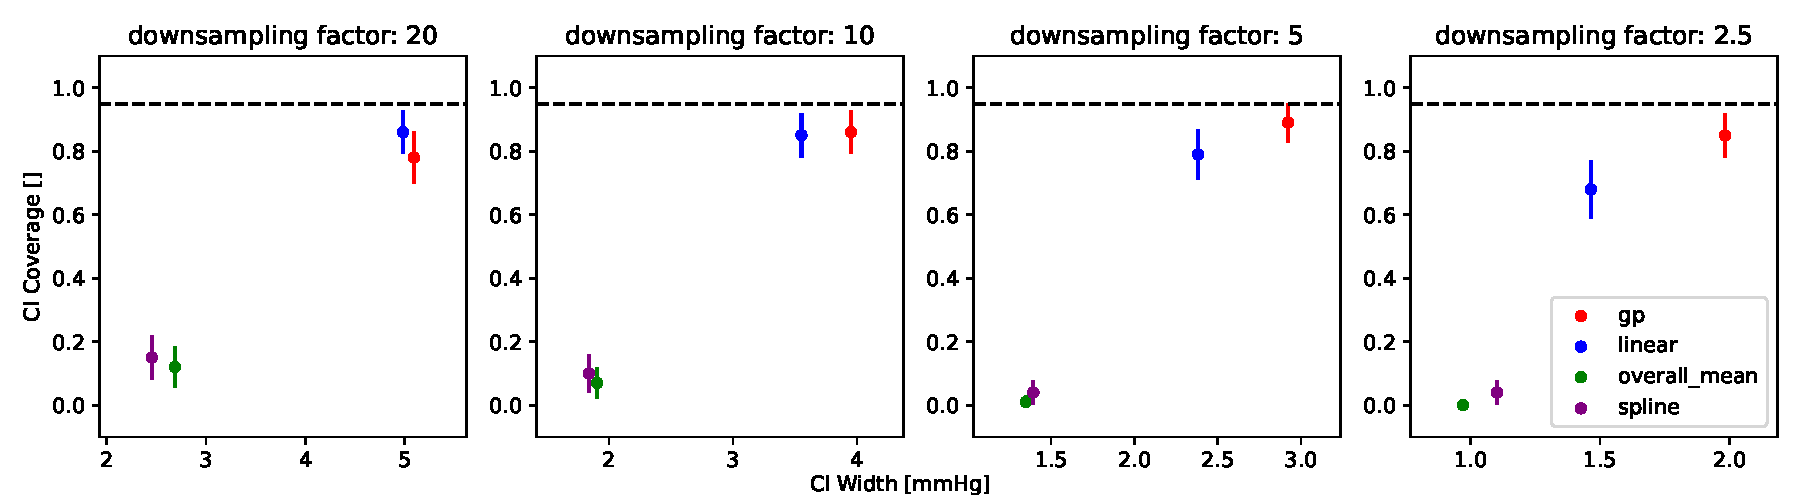
\includegraphics[width=\linewidth]{Pictures/final_experiment_hpdi/overall_mean_eval_sin_rbf_seasonal_extreme}
    \caption{One-Week Mean - Extreme Seasonal Downsampling}
    \label{fig:weekly-mean-extreme-seasonal-sampling-performance}
\end{subfigure}

\caption[One-Week Mean Performance]{
    Performance comparison of various methods for
estimating the one-week mean across different downsampling patterns.
    The dashed horizontal line indicates the target CI coverage of 95\%.
}
\label{fig:weekly-mean-performance}
\end{figure}



\subsection{One-Day and One-Hour Mean}

Figures \ref{fig:daily-mean-performance} and \ref{fig:hourly-mean-performance}
illustrate the performance of different methods in estimating the one-day and one-hour mean,
respectively, based on various downsampling patterns.

GP regression consistently produces the best estimates for both the one-hour and
one-day mean across all sampling patterns.
Its superiority becomes more pronounced with increased data availability and
an increasing amount of seasonal sampling.

Spline regression, when not suffering from the estimation instability
described in the previous subsection, also yields decent results.
In the case of uniform sampling, the one-day mean is adequately approximated
by the naive TTR method.

However, linear regression does not appear to produce accurate estimates for
either the one-day or one-hour mean, regardless of the sampling pattern.


\begin{figure}[!htb]
\centering
\begin{subfigure}{\textwidth}
    \centering
    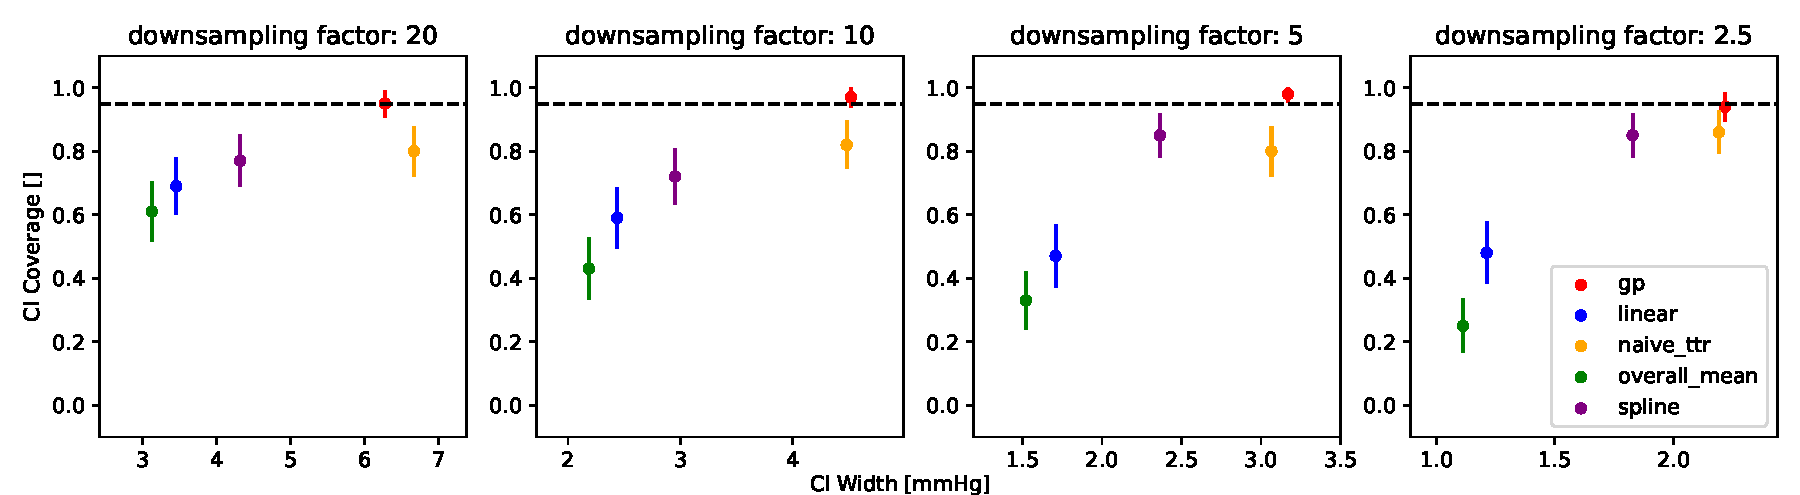
\includegraphics[width=\linewidth]{Pictures/final_experiment_hpdi/mean_24h_eval_sin_rbf_default}
    \caption{One-Day Mean Performance - Uniform Downsampling}
    \label{fig:daily-mean-uniform-sampling-performance}
\end{subfigure}

\bigskip

\begin{subfigure}{\textwidth}
    \centering
    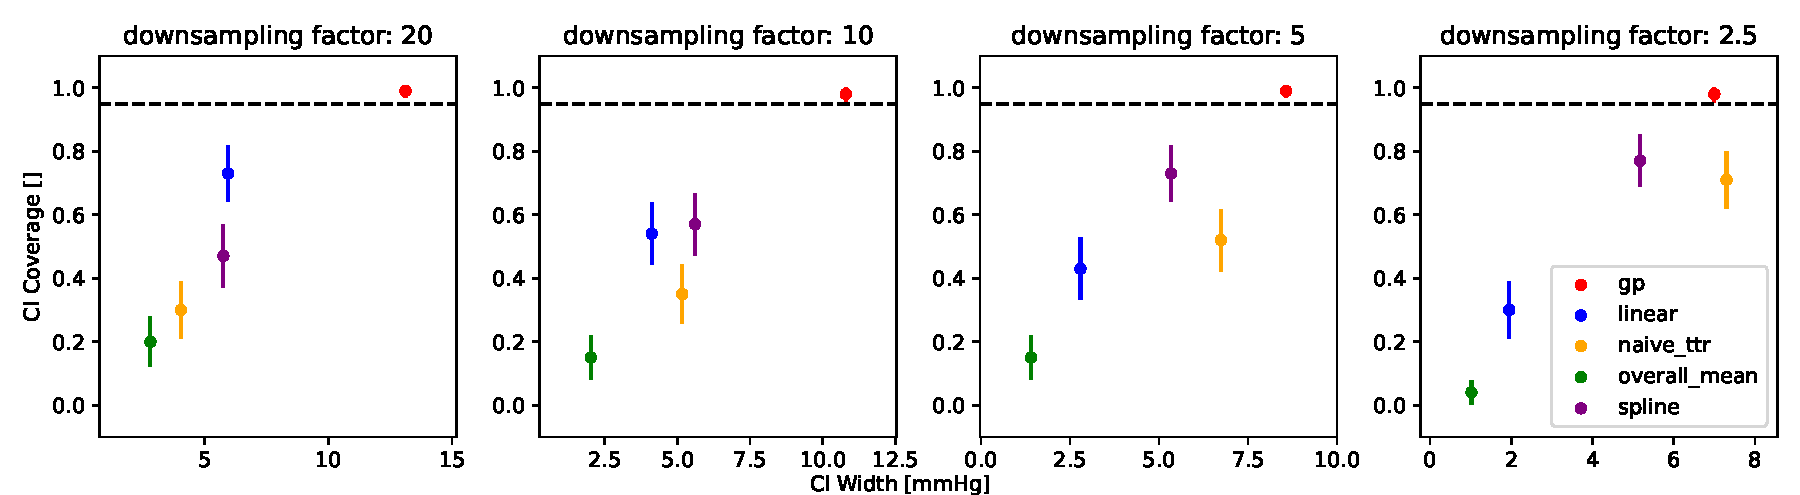
\includegraphics[width=\linewidth]{Pictures/final_experiment_hpdi/mean_1h_eval_sin_rbf_seasonal_default}
    \caption{One-Day Mean Performance - Seasonal Downsampling}
    \label{fig:daily-mean-seasonal-sampling-performance}
\end{subfigure}

\bigskip

\begin{subfigure}{\textwidth}
    \centering
    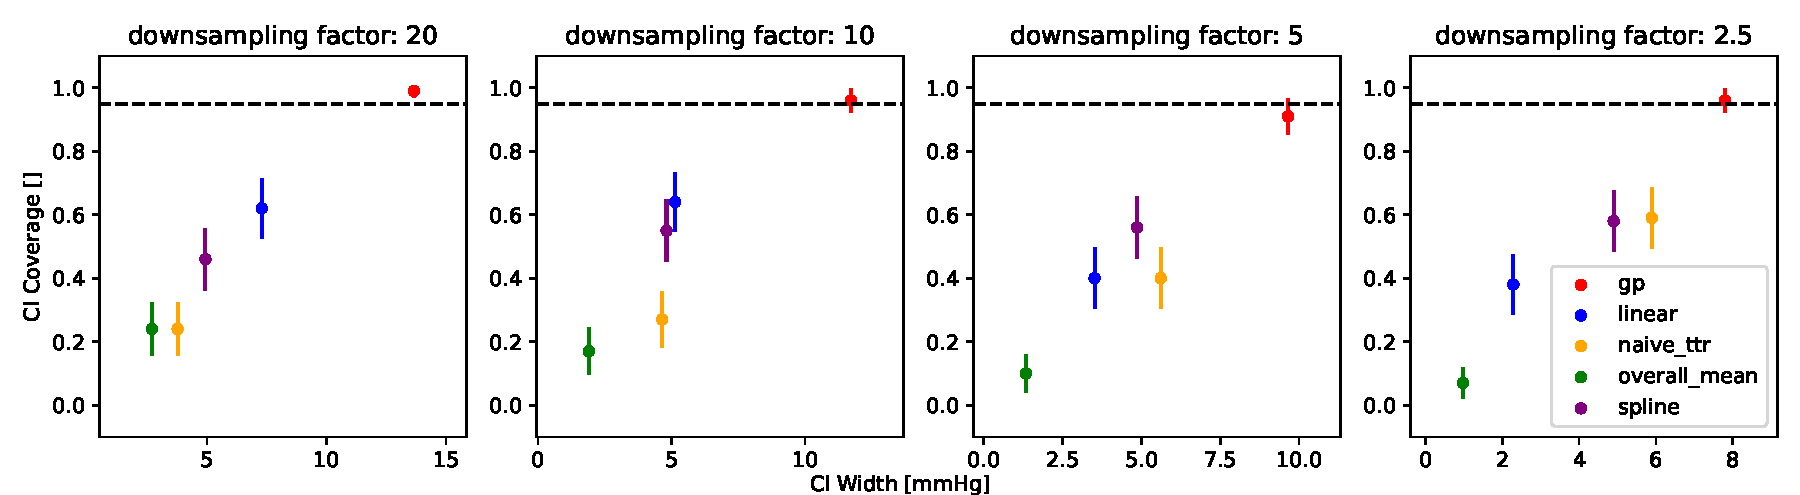
\includegraphics[width=\linewidth]{Pictures/final_experiment_hpdi/mean_1h_eval_sin_rbf_seasonal_extreme}
    \caption{One-Day Mean Performance - Extreme Seasonal Downsampling}
    \label{fig:daily-mean-extreme-seasonal-sampling-performance}
\end{subfigure}

\caption[One-Day Mean Performance]{
Performance comparison of various methods for
estimating the one-day mean across different downsampling patterns.
The dashed horizontal line indicates the target CI coverage of 95\%.

}
\label{fig:daily-mean-performance}
\end{figure}




\begin{figure}[!htb]
\centering
\begin{subfigure}{\textwidth}
    \centering
    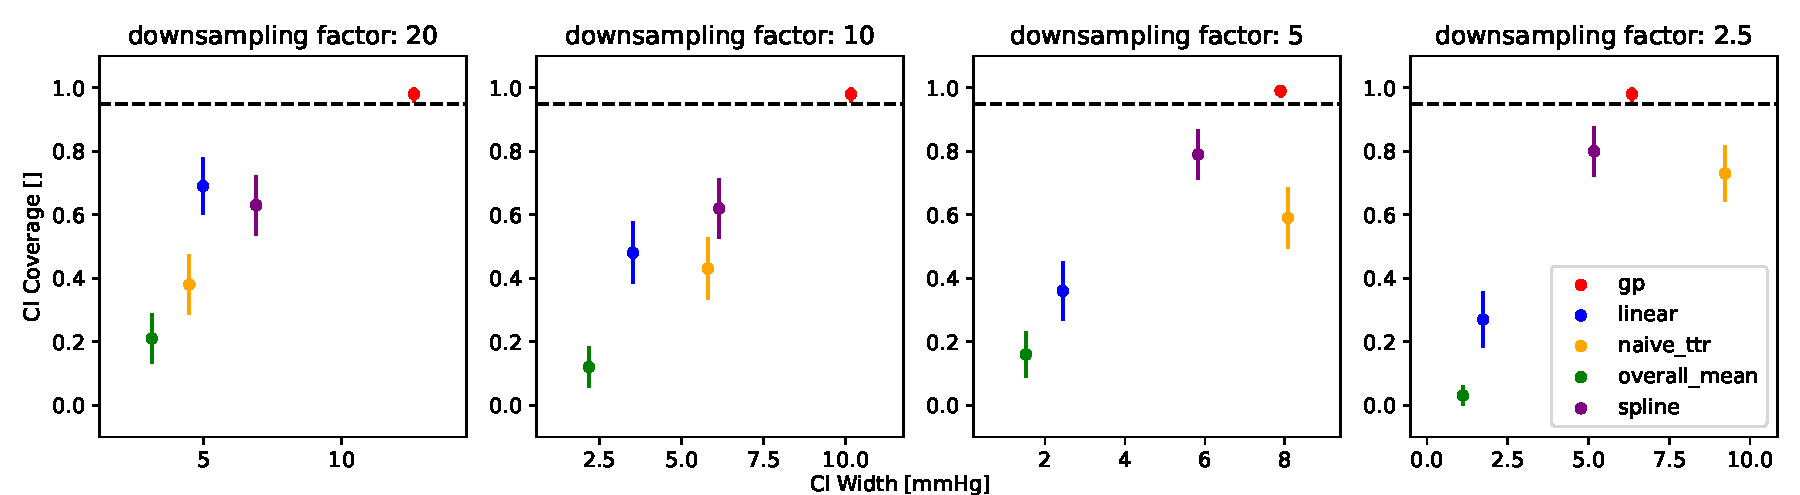
\includegraphics[width=\linewidth]{Pictures/final_experiment_hpdi/mean_1h_eval_sin_rbf_default}
    \caption{One-Hour Mean Performance - Uniform Downsampling}
    \label{fig:hourly-mean-uniform-sampling-performance}
\end{subfigure}

\bigskip

\begin{subfigure}{\textwidth}
    \centering
    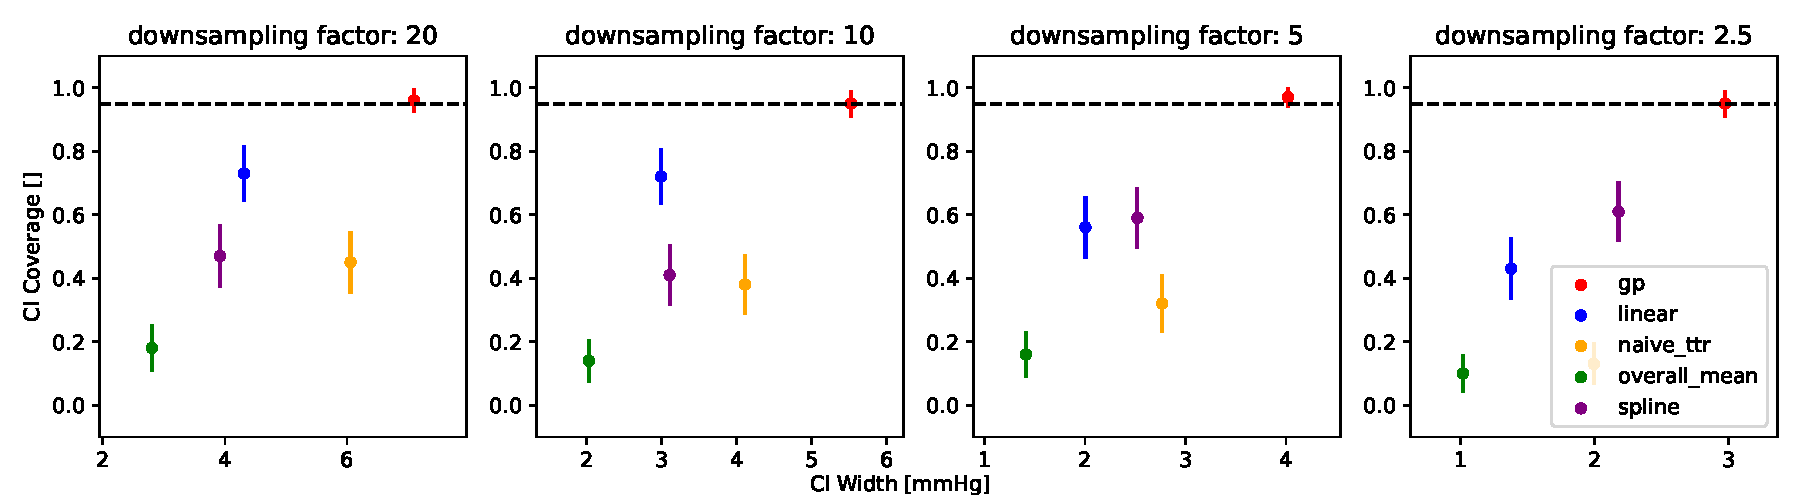
\includegraphics[width=\linewidth]{Pictures/final_experiment_hpdi/mean_24h_eval_sin_rbf_seasonal_default}
    \caption{One-Hour Mean Performance - Seasonal Downsampling}
    \label{fig:hourly-mean-seasonal-sampling-performance}
\end{subfigure}

\bigskip

\begin{subfigure}{\textwidth}
    \centering
    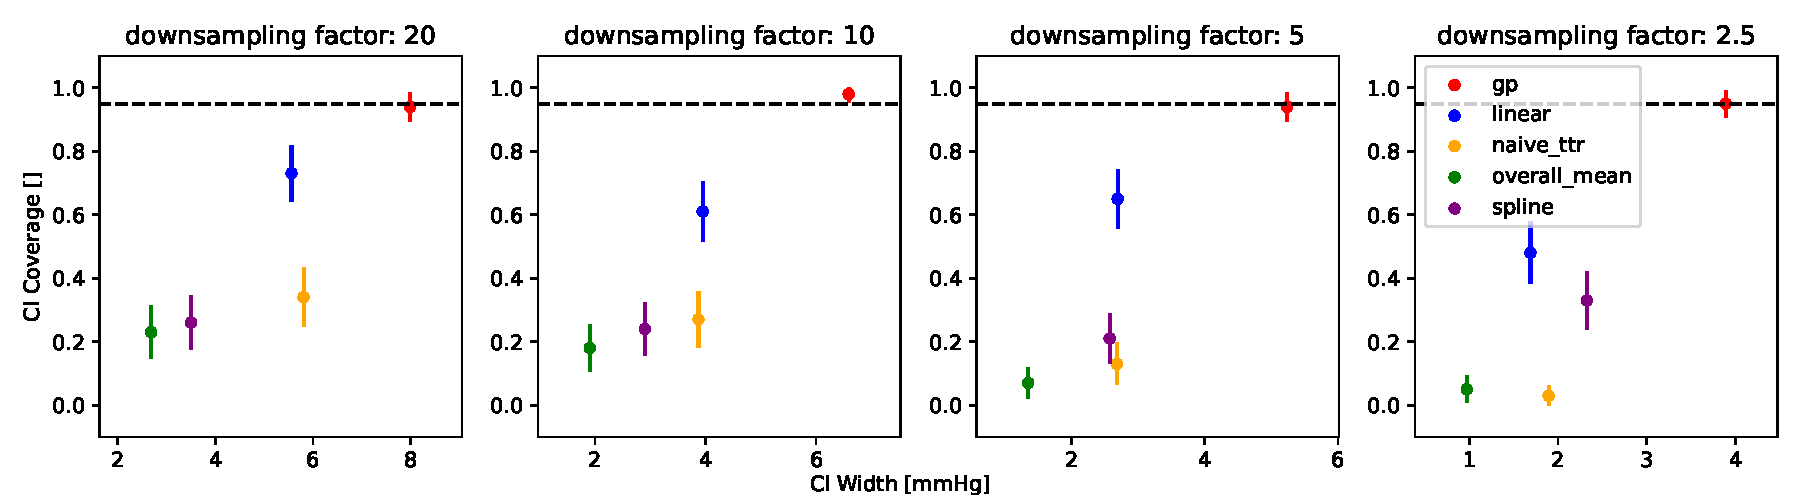
\includegraphics[width=\linewidth]{Pictures/final_experiment_hpdi/mean_24h_eval_sin_rbf_seasonal_extreme}
    \caption{One-Hour Mean Performance - Extreme Seasonal Downsampling}
    \label{fig:hourly-mean-extreme-seasonal-sampling-performance}
\end{subfigure}

\caption[One-Hour Mean Performance]{Performance comparison of various methods for
estimating the one-hour mean across different downsampling patterns.
The dashed horizontal line indicates the target CI coverage of 95\%.

}
\label{fig:hourly-mean-performance}
\end{figure}


\subsection{Time in Target Range}\label{subsec:time-in-target-range}

Figure \ref{fig:ttr-performance} displays the performance of different methods
in estimating TTR based on various downsampling patterns.
Among these methods, GP regression stands out as the only one consistently achieving
adequate CI coverage for most of the downsampling patterns.
While spline regression comes close, particularly with uniform sampling and
large downsampling factors, GP regression consistently yields narrower CIs.
It is important to note that TTR does not depend on the absolute values of the blood pressure (BP)
estimates but rather focuses on whether these estimates fall within the target range.
As TTR is not affected by extreme estimate values occasionally produced by spline regression,
this method provides reasonable TTR estimates.
However, the current approach used for estimating TTR ("naive\_ttr") performs poorly.
This is because it does not estimate TTR through the estimation of $f(x)$ but directly
operates on the noisy measurements $Y(x)$. As a result, it generally underestimates TTR.


\begin{figure}[!htb]
\centering
\begin{subfigure}{\textwidth}
    \centering
    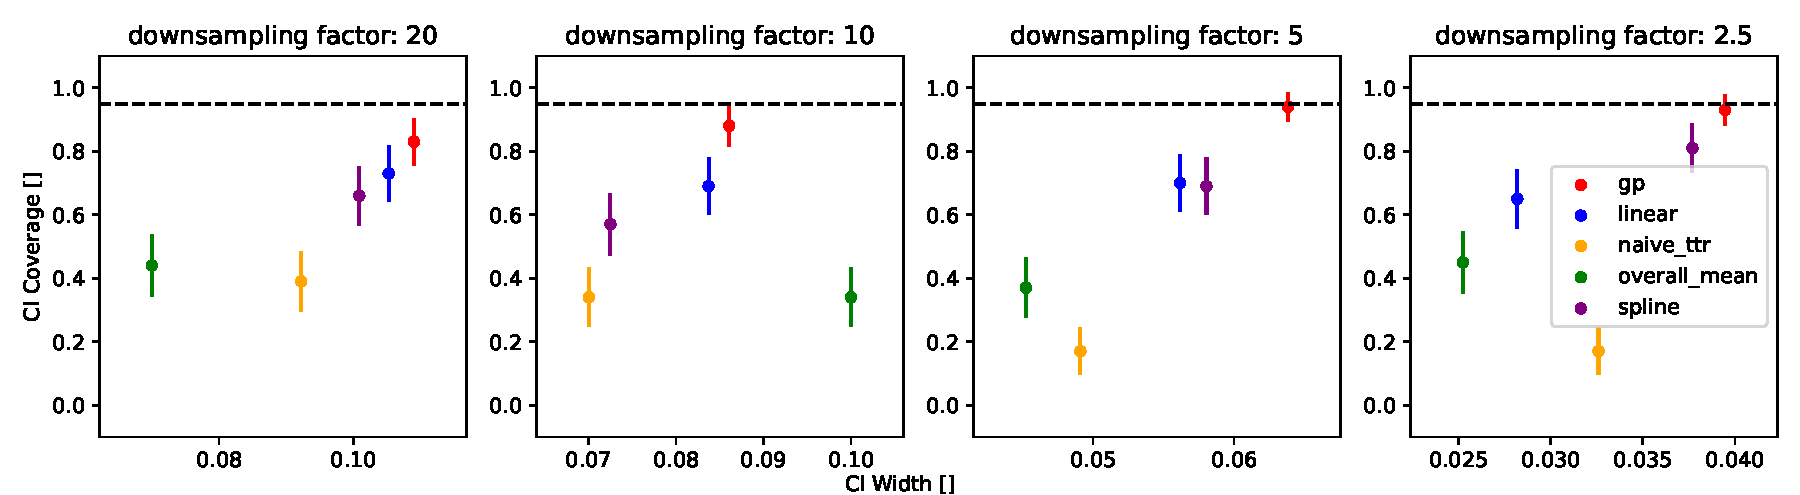
\includegraphics[width=\linewidth]{Pictures/final_experiment_hpdi/ttr_eval_sin_rbf_default}
    \caption{TTR Performance - Uniform Downsampling}
    \label{fig:ttr-uniform-sampling-performance}
\end{subfigure}

\bigskip

\begin{subfigure}{\textwidth}
    \centering
    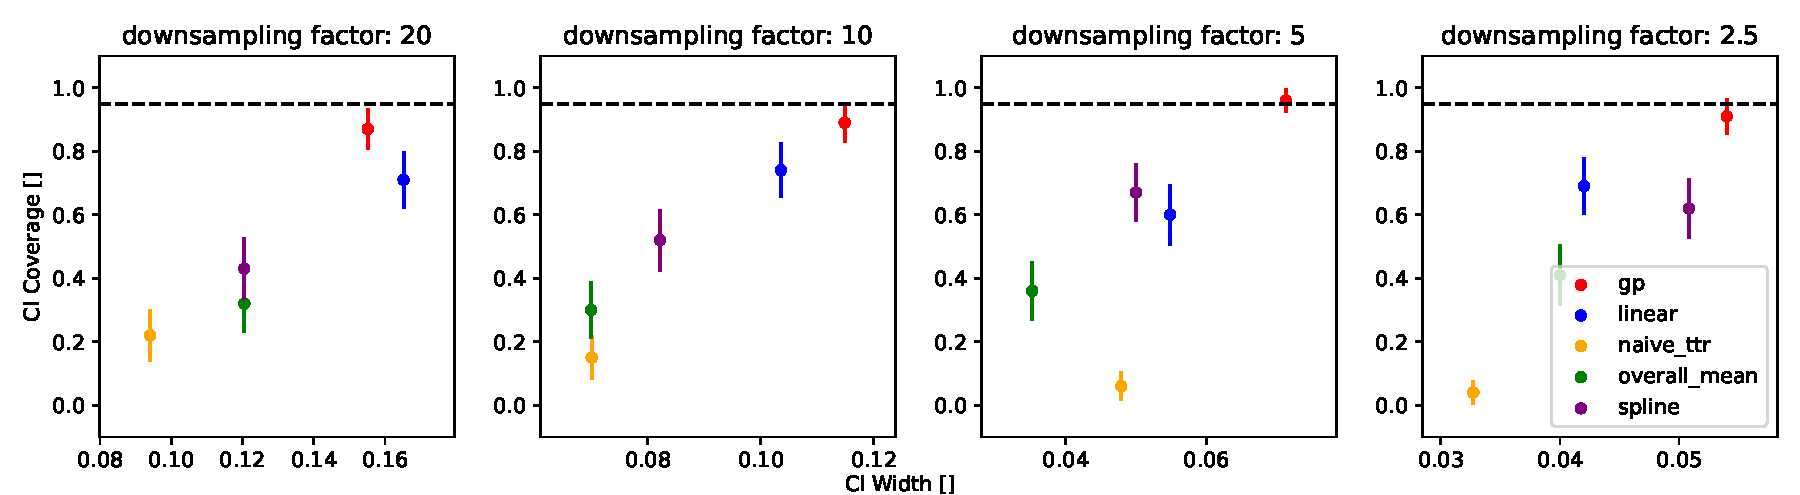
\includegraphics[width=\linewidth]{Pictures/final_experiment_hpdi/ttr_eval_sin_rbf_seasonal_default}
    \caption{TTR Performance - Seasonal Downsampling}
    \label{fig:ttr-seasonal-sampling-performance}
\end{subfigure}

\bigskip

\begin{subfigure}{\textwidth}
    \centering
    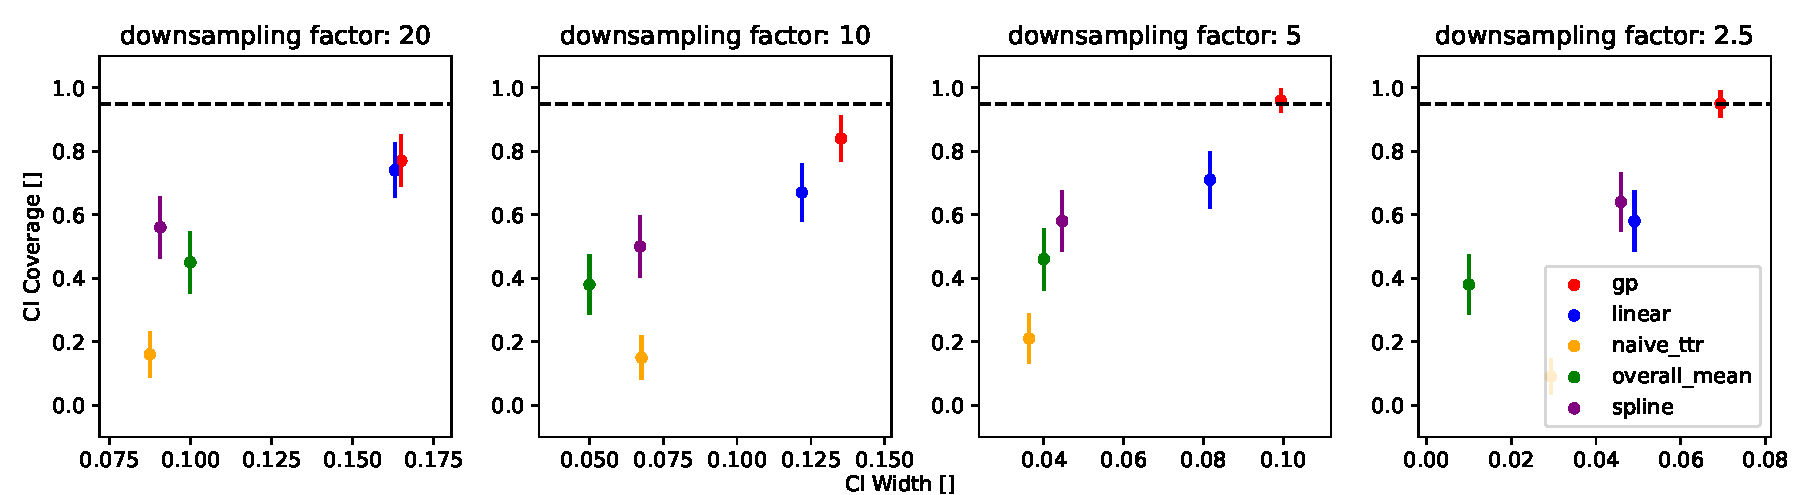
\includegraphics[width=\linewidth]{Pictures/final_experiment_hpdi/ttr_eval_sin_rbf_seasonal_extreme}
    \caption{TTR Performance - Extreme Seasonal Downsampling}
    \label{fig:ttr-extreme-seasonal-sampling-performance}
\end{subfigure}

\caption[TTR Performance]{Performance comparison of various methods for
estimating TTR across different downsampling patterns.
The dashed horizontal line indicates the target CI coverage of 95\%.
}
\label{fig:ttr-performance}
\end{figure}


\section{Examples}
This section presents illustrative examples to support the observations made in
the preceding section.


\subsection{Impact of Downsampling Factor}


Figure \ref{fig:ex-downsampling-factor} provides an example of how various
methods perform as more data is incorporated. In this context:

\begin{itemize}
    \item Linear regression demonstrates the ability to produce accurate estimates even
    at high downsampling factors. However, unlike GP regression, it does not exhibit
    substantial improvement as more data is included.
    \item Conversely, GP regression displays notable improvements with an
    increasing amount of data.
    \item Spline regression , on the other hand, struggles to capture the cyclic
    component due to the prominent presence of an AR component, even when a
    substantial amount of data is available.
\end{itemize}

\begin{figure}
\begin{subfigure}{\textwidth}
    \centering
    \includegraphics[width=0.45\linewidth]{
       Pictures/plots_final6/sin_rbf_default_0.05/09_14_11_12_35/plot_posterior_confint_spline.pdf}
    \includegraphics[width=0.45\linewidth]{
      Pictures/plots_final6/sin_rbf_default_0.4/09_14_13_25_16/plot_posterior_confint_spline.pdf}
  \caption{Spline Regression }
\end{subfigure}

\begin{subfigure}{\textwidth}
    \centering
    \includegraphics[width=.45\linewidth]{
       Pictures/plots_final6/sin_rbf_default_0.05/09_14_11_12_35/plot_posterior_confint_linear.pdf}
    \includegraphics[width=0.45\linewidth]{
  Pictures/plots_final6/sin_rbf_default_0.4/09_14_13_25_16/plot_posterior_confint_linear.pdf}
  \caption{Linear regression }
\end{subfigure}

\begin{subfigure}{\textwidth}
    \centering
    \includegraphics[width=0.45\linewidth]{
       Pictures/plots_final6/sin_rbf_default_0.05/09_14_11_12_35/plot_posterior_confint_gp.pdf}
    \includegraphics[width=0.45\linewidth]{
  Pictures/plots_final6/sin_rbf_default_0.4/09_14_13_25_16/plot_posterior_confint_gp.pdf}
  \caption{GP regression}
\end{subfigure}\hfill

\caption[Impact of Downsampling Factor]{Impact of Downsampling Factor:
    Estimated BP values $\hat{f}(x)$ (black) and corresponding confidence intervals
    (gray area) based on measurements (purple dots) using various methods.
    Measurments have been obtained using a
    downsampling factor of 20 (left panels) and 2.5 (right panels).
    The true BP values, $f(x)$, (red dotted line) are the same in all shown
    scenarios however the range of values shown on the y-axis varies.
    }
\label{fig:ex-downsampling-factor}
\end{figure}

\subsection{Seasonal Samping and Downsampling Factor}




Figure \ref{fig:ex-seasonal-sampling} illustrates the influence of different
downsampling factors in the presence of extreme seasonal sampling on the estimated
BP values and CIs. In this context:
\begin{itemize}
    \item Linear regression once again demonstrates its ability to produce
    reasonably accurate results when only limited data is available.
    However, its performance does not see substantial improvement as more data is introduced.
    Interestingly, as more data is incorporated, linear regression tends to underestimate uncertainty,
    resulting in reduced CI coverage.
    \item On the contrary, spline regression does not provide very accurate estimates
    for the BP values. Nevertheless, the CIs it generates are wide enough to maintain
    adequate coverage.
    Predictions tend to improve with increased data, particularly at the peaks
    where data density is higher than in the valleys.
    Notably, spline regression does not prioritize fitting a cyclic pattern,
    resulting in higher uncertainty estimates in the valleys compared to those
    produced by GP regression and linear regression.
    \item GP regression primarily improves by narrowing the CI width as more data is added.
    Importantly, unlike linear regression, the CIs generated by GP regression continue
    to cover the true BP values.
\end{itemize}


\begin{figure}
\begin{subfigure}{\textwidth}
    \centering
    \includegraphics[width=0.45\linewidth]{
    Pictures/plots_final6/sin_rbf_seasonal_extreme_0.05/09_14_11_49_06/plot_posterior_confint_spline.pdf}
    \includegraphics[width=0.45\linewidth]{
    Pictures/plots_final6/sin_rbf_seasonal_extreme_0.4/09_14_14_12_40/plot_posterior_confint_spline.pdf}
  \caption{Spline Regression}
\end{subfigure}

\begin{subfigure}{\textwidth}
    \centering
    \includegraphics[width=.45\linewidth]{
    Pictures/plots_final6/sin_rbf_seasonal_extreme_0.05/09_14_11_49_06/plot_posterior_confint_linear.pdf}
    \includegraphics[width=0.45\linewidth]{
        Pictures/plots_final6/sin_rbf_seasonal_extreme_0.4/09_14_14_12_40/plot_posterior_confint_linear.pdf}
  \caption{Linear regression }
\end{subfigure}

\begin{subfigure}{\textwidth}
    \centering
    \includegraphics[width=0.45\linewidth]{
    Pictures/plots_final6/sin_rbf_seasonal_extreme_0.05/09_14_11_49_06/plot_posterior_confint_gp.pdf}
    \includegraphics[width=0.45\linewidth]{
       Pictures/plots_final6/sin_rbf_seasonal_extreme_0.4/09_14_14_12_40/plot_posterior_confint_gp.pdf}
  \caption{GP regression}
\end{subfigure}\hfill

\caption[Seasonal Samping and Downsampling Factor]{Seasonal Samping and Downsampling Factor:
    Estimated BP values $\hat{f}(x)$ (black) and corresponding confidence intervals (gray area)
    based on measurements (purple dots) using various methods.
    The measurements were obtained through extreme seasonal sampling with downsampling
    factors of 20 (left panels) and 2.5 (right panels).
    The true BP values, $f(x)$, are represented by the red dotted line.}
\label{fig:ex-seasonal-sampling}
\end{figure}



\subsection{Dominant Cyclic Component vs. Dominant AR Component}
\label{subsec:dominant-cyclic-component-vs-dominant-ar-component}

Figure \ref{fig:ex-ar-cyclic} presents a comparison of predictions under two
scenarios: when the AR component dominates and when the cyclic component takes precedence. In this context:

\begin{itemize}
    \item When the cyclic component dominates, all methods perform well and
    provide accurate predictions also for a large downsampling factor of 10.
    \item However, when the AR component is predominant:

    \begin{itemize}
        \item  Only GP regression is capable of offering reliable local BP value estimates.
        Nevertheless, in scenarios with limited data availability, GP regression tends to overemphasize the influence of
        the AR component while underestimating the contribution from the cyclic component.
        This behavior is depicted in sub-figure \ref{subfig:mean-decomposed-ar}.
        Due to the flexibility of the kernels used, they may occasionally capture features originating from another kernel.
        \item Linear regression, on the other hand, is constrained
        to predict a perfect sinusoid with a linear trend.
        Consequently, it struggles to fit the AR component effectively,
        even when data availability is high (downsampling factor of 2.5), which leads to inaccurate predictions.
        Additionally, it underestimates uncertainty in such cases.
    \end{itemize}
\end{itemize}


\begin{figure}
\begin{subfigure}{\textwidth}
    \centering
    \includegraphics[width=0.45\linewidth]{
    Pictures/plots_final6/sin_rbf_default_0.1/09_14_11_57_29/plot_true_mean_decomposed.pdf}
    \includegraphics[width=0.45\linewidth]{
    Pictures/plots_final6/sin_rbf_default_0.4/09_14_13_34_15/plot_true_mean_decomposed.pdf}
  \caption{Decompositon of $f(x)$: The cyclic component is shown in orange, the AR component in blue.}
\end{subfigure}

\begin{subfigure}{\textwidth}
    \centering
    \includegraphics[width=0.45\linewidth]{
    Pictures/plots_final6/sin_rbf_default_0.1/09_14_11_57_29/plot_posterior_confint_spline.pdf}
    \includegraphics[width=0.45\linewidth]{
        Pictures/plots_final6/sin_rbf_default_0.4/09_14_13_34_15/plot_posterior_confint_spline.pdf}
  \caption{Spline Regression }
\end{subfigure}

\begin{subfigure}{\textwidth}
    \centering
    \includegraphics[width=.45\linewidth]{
    Pictures/plots_final6/sin_rbf_default_0.1/09_14_11_57_29/plot_posterior_confint_linear.pdf}
    \includegraphics[width=0.45\linewidth]{
        Pictures/plots_final6/sin_rbf_default_0.4/09_14_13_34_15/plot_posterior_confint_linear.pdf}
  \caption{Linear regression }
\end{subfigure}

\begin{subfigure}{\textwidth}
    \centering
    \includegraphics[width=0.45\linewidth]{
    Pictures/plots_final6/sin_rbf_default_0.1/09_14_11_57_29/plot_posterior_confint_gp.pdf}
    \includegraphics[width=0.45\linewidth]{
        Pictures/plots_final6/sin_rbf_default_0.4/09_14_13_34_15/plot_posterior_confint_gp.pdf}
  \caption{GP regression}
\end{subfigure}\hfill
\caption[Dominant Cyclic Component vs. Dominant AR Component]{
Dominant Cyclic Component vs. Dominant AR Component:
    Estimated BP values $\hat{f}(x)$ (black) and corresponding confidence intervals (gray area)
    based on measurements (purple dots) using various methods.
    The measurements were uniformly sampled with a downsampling factor of 5.
    The true BP values, $f(x)$, are depicted by the red dotted line.
    The right panels show BP value predictions under a prominent AR component and with a dwonsampling factor of 2.5,
    while the left panels display predictions under a prominent cyclic component and with a downsampling factor of 10.
 }
\label{fig:ex-ar-cyclic}
\end{figure}



\begin{figure}

\begin{subfigure}{\textwidth}
    \centering
    \includegraphics[width=0.66\linewidth]{
    Pictures/plots_final6/sin_rbf_default_0.1/09_14_11_57_29/plot_mean_decomposed_vertical}
    \includegraphics[width=0.33\linewidth]{
    Pictures/plots_final6/sin_rbf_default_0.1/09_14_11_57_29/plot_posterior_confint_gp.pdf}
  \caption{Dominant Cyclic Component - Downsampling Factor of 10}
\end{subfigure}

\begin{subfigure}{\textwidth}
    \centering
    \includegraphics[width=0.66\linewidth]{
        Pictures/plots_final6/sin_rbf_default_0.4/09_14_13_34_15/plot_mean_decomposed_vertical}
    \includegraphics[width=0.33\linewidth]{
         Pictures/plots_final6/sin_rbf_default_0.4/09_14_13_34_15/plot_posterior_confint_gp.pdf}
  \caption{Dominant AR Component - Downsampling Factor of 2.5}
    \label{subfig:mean-decomposed-ar-low-downsampling}
\end{subfigure}\hfill

\begin{subfigure}{\textwidth}
    \centering
    \includegraphics[width=0.66\linewidth]{
    Pictures/plots_final6/sin_rbf_default_0.2/09_14_12_47_04/plot_mean_decomposed_vertical}
    \includegraphics[width=0.33\linewidth]{
       Pictures/plots_final6/sin_rbf_default_0.2/09_14_12_47_04/plot_posterior_confint_gp}
  \caption{Dominant AR Component - Downsampling Factor of 5}
    \label{subfig:mean-decomposed-ar}
\end{subfigure}\hfill
\label{fig:mean-decomposed-ar-cyclic}
\caption[Dominant Cyclic Component vs. Dominant AR Component: Decomposition of $f(x)$]{
    The left panels display the decomposition of the true BP values $f(x)$.
    The middle panels illustrate the decomposition of the estimated BP values $\hat{f}(x)$.
    The cyclic component is represented in orange,
    the AR component in blue, and the long-term trend in green.
    When the cyclic component is dominant, fewer data points are required to obtain accurate BP estimates
    compared to when the AR component is dominant.
    In the case of a dominant AR component, GP regression tends to underestimate
    the contribution from the cyclic component.
    When using a downsampling factor of 5, GP regression also tends to overestimate
    the variance associated with the AR component.
}

\end{figure}

\subsection{Spline Regression  Failure}

Figure \ref{fig:ex-spline-failure} provides a visualization of how
spline regression generates exceptionally large CIs when
applied under high downsampling factors.
In such scenarios, bootstrapping produces highly unstable BP estimates.
This phenomenon becomes evident when observing the results of a single bootstrap
sample in these conditions, as demonstrated in subfigure \ref{subfig:ex-spline-failure-bootstrap}.
Note, that the one-week, one-day, and one-hour means derived from this single bootstrap sample
would be considerably underestimated.
However, TTR estimates might still be reasonable.

\begin{figure}[!htb]
\centering
\begin{subfigure}{.5\textwidth}
    \centering
    \includegraphics[width=\linewidth]{Pictures/spline_extreme/plot_posterior_confint_spline}
    \caption{Spline Regression  PB estimates (black line) with corresponding CIs (gray area),
        both obtained through bootstrapping.
        Additionally, the true BP values (red dotted line) are displayed along
        with the training samples (red dots).}
\end{subfigure}\hfill
\begin{subfigure}{.42\textwidth}
    \centering
    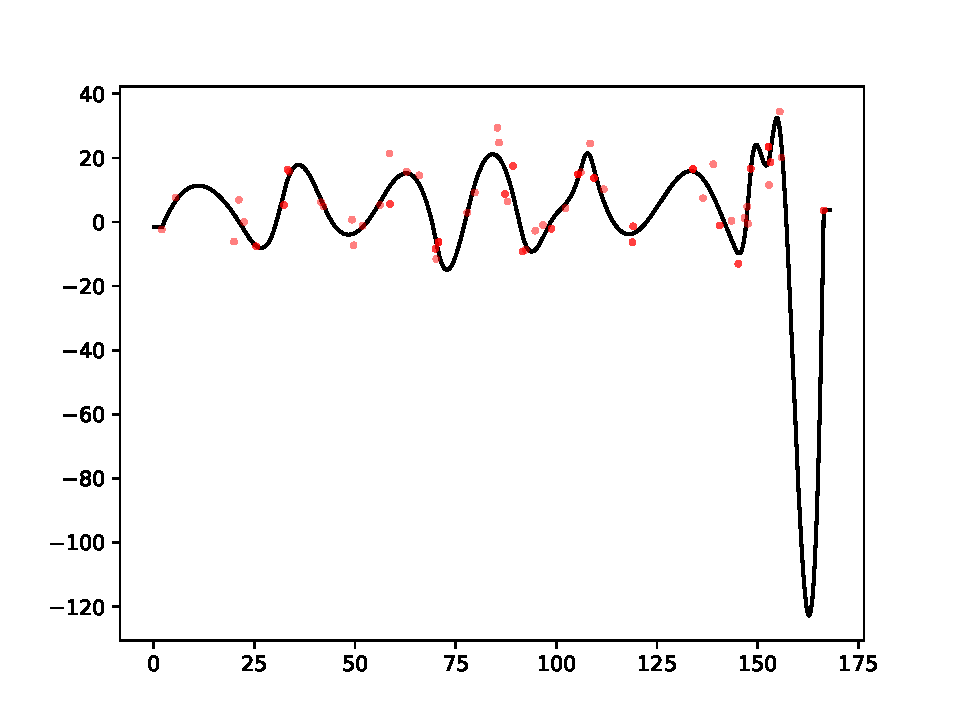
\includegraphics[width=\linewidth]{Pictures/spline_extreme/plot_pred_bootstrap_spline_reg_v2_70}
  \caption[Estimate Single Bootstrap Sample]{
      BP value estimates (black line) based on samples of one bootstrap iteration (red dots).
      \\
        \\}
    \label{subfig:ex-spline-failure-bootstrap}
\end{subfigure}
\caption[Spline Regression  Failure]{
    Spline Regression  Failure:
    Spline regression  generates extreme local BP value predictions
    under a downsampling factor of 20.
    Such BP value drops as shown in Panel (b) result in
    the generation of exceptionally
    large confidence intervals in certain regions (Panel (a)).}
\label{fig:ex-spline-failure}
\end{figure}






%\begin{example}
%
%\begin{figure}[!htb]
%\centering
%\includegraphics[width=\linewidth]{Pictures/plots_final2/sin_rbf_default_0.2/09_11_07_49_51/plot_posterior}
%\caption[GP Prediction]{Predictive mean of $F_{X}$ (blackline) with
%predictive variance (grey area) based on observations (purple dots) }
%\label{fig:ex1-gp-prediction}
%\end{figure}
%
%\begin{figure}[!htb]
%\centering
%\includegraphics[width=\linewidth]{Pictures/plots_final2/sin_rbf_default_0.2/09_11_07_49_51/plot_mean_decomposed}
%\caption[Mean Decomposed Predicted vs True]{Each figure shows one sample $F_X$ drawn from the true GP (red dashed line) with noisy observations
%  (purple dots) sampled at a frequency of 0.5/hour}
%\label{fig:ex1-gp-mean-decomposed}
%\end{figure}
%
%
%\begin{figure}[!htb]
%\centering
%\begin{subfigure}{.45\textwidth}
%    \centering
%    \includegraphics[width=\linewidth]{Pictures/plots_final2/sin_rbf_default_0.2/09_11_07_49_51/plot_posterior_spline}
%  \caption[Spline]{The sample $F_X$ shown to the right, decomposed in to the contribution of the Periodic kernel (orange),
%      Matérn kernel (blue), RBF kernel (green).}
%  \label{fig:ex1-spline}
%\end{subfigure}\hfill
%\begin{subfigure}{.45\textwidth}
%    \centering
%    \includegraphics[width=\linewidth]{Pictures/plots_final2/sin_rbf_default_0.2/09_11_07_49_51/plot_posterior_linear}
%  \caption[Linear Regression]{Each figure shows one sample $F_X$ drawn from the true GP (red dashed line) with noisy observations
%      (purple dots) sampled at a frequency of 0.5/hour}
%  \label{fig:ex1-linear}
%\end{subfigure}
%\caption[Baseline Methods]{Baseline Methods Example Prediction}
%\label{fig:ex1}
%\end{figure}
%



%\end{example}









